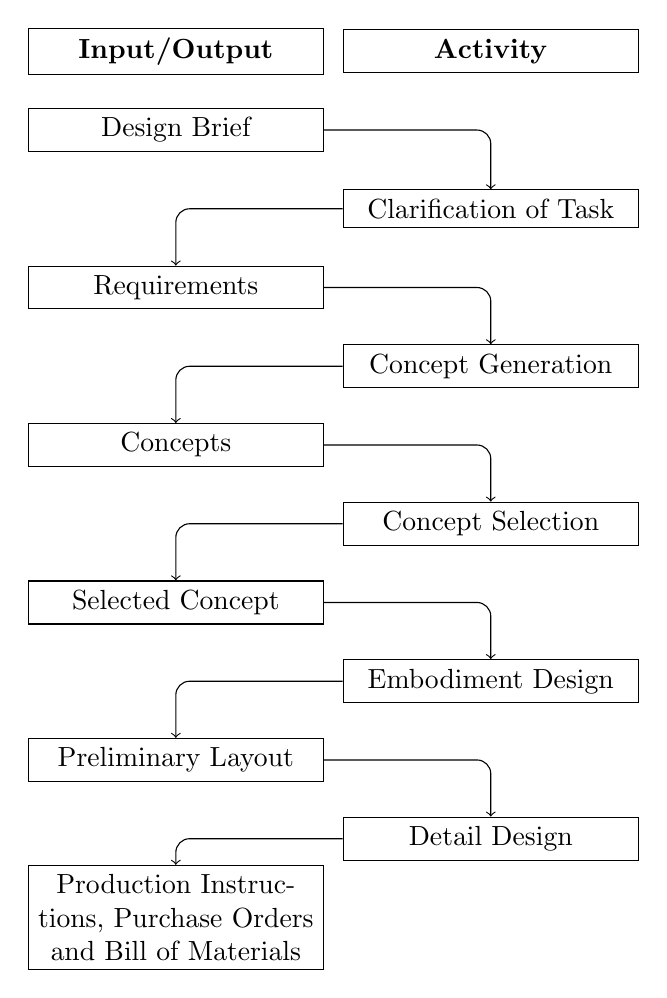
\begin{tikzpicture}
  %\node[draw, text width=100, align=center] (N) at (-4,0) {\textbf{Study Week}};
  \node[draw, text width=100, align=center] (A) at (0,0) {\textbf{Input/Output}};
  \node[draw, text width=100, align=center] (B) at (4,0) {\textbf{Activity}};


  \node[draw, text width=100, align=center] (C) at (0,-1) {Design Brief};

  \node[draw, text width=100, align=center] (D) at (4,-2) {Clarification of Task};
  \draw[->, rounded corners=5pt] (C) -| (D);

  \node[draw, text width=100, align=center] (E) at (0,-3) {Requirements};
  \draw[->, rounded corners=5pt] (D) -| (E);

  \node[draw, text width=100, align=center] (F) at (4,-4) {Concept Generation};
  \draw[->, rounded corners=5pt] (E) -| (F);

  \node[draw, text width=100, align=center] (G) at (0,-5) {Concepts};
  \draw[->, rounded corners=5pt] (F) -| (G);

  \node[draw, text width=100, align=center] (H) at (4,-6) {Concept Selection};
  \draw[->, rounded corners=5pt] (G) -| (H);

  \node[draw, text width=100, align=center] (I) at (0,-7) {Selected Concept};
  \draw[->, rounded corners=5pt] (H) -| (I);

  \node[draw, text width=100, align=center] (J) at (4,-8) {Embodiment Design};
  \draw[->, rounded corners=5pt] (I) -| (J);

  \node[draw, text width=100, align=center] (K) at (0,-9) {Preliminary Layout};
  \draw[->, rounded corners=5pt] (J) -| (K);

  \node[draw, text width=100, align=center] (L) at (4,-10) {Detail Design};
  \draw[->, rounded corners=5pt] (K) -| (L);

  \node[draw, text width=100, align=center] (M) at (0,-11) {Production Instructions, Purchase Orders and Bill of Materials};
  \draw[->, rounded corners=5pt] (L) -| (M);


\end{tikzpicture}